\section{Today's assignment}
Today's class will be divided in two main parts. Firstly, we will learn about
computation graphs and the Backpropagation algorithm. We will also code
Backpropagation in Numpy for a simple model (a feed forward network). Secondly,
we will learn the basics of the Theano module for Python. Theano allows you to
implement  generic computation graphs, automatically compute gradients with
respect to their parameters and make use of Graphical Processing Units (GPUs)
for optimal speed. 

If you are new to the topic, you should aim to understand the concept of computation graph, 
finish the Backpropagation exercise and attain a basic understanding of Theano.
If you already know Backpropagation well and have experience with normal
Python, you should aim to complete the whole day. 

\section{Introduction to Deep Learning and Theano}

Deep learning is the name behind the latest wave of neural network research.
This is a very old topic, dating from the first half of the 20th century, that
has attained formidable impact in the machine learning community recently. 
There is nothing particularly difficult in deep learning. You have already
visited all the mathematical principles you need in the first days of the
labs of this school. At their core, deep learning models are just functions
mapping vector inputs $\mathbf{x}$ to vector outputs $\mathbf{y}$, constructed by
composing linear and non-linear functions. This composition can be expressed in
the form of a \textit{computation graph}, where each node applies a function to
its inputs and passes the result as its output. The parameters of the model are
the weights given to the different inputs in nodes applying linear
functions. This resembles vaguely synapse strengths in human neural networks,
hence the name artificial neural networks. 

Due to their compositional nature, gradient methods and the chain rule can be
applied learn the parameters of these models regardless of their complexity.
See Section \label{gradient_methods} for a refresh on the basic concept. We
will also refer to the gradient learning methods introduced in Section
\ref{s:me}. Today we will focus on \textit{feed-forward networks}. we will
extended today's class to \textit{recurrent neural networks} (RNNs).  

Some of the changes that led to the surge of deep learning are not only
improvements on the existing neural network algorithms, but also
the increase in the amount of data available and computing power. In
particular, the use of Graphical Processing Units (GPUs) has allowed neural
networks to be applied to very large datasets. Working with GPUs is not trivial
as it requires dealing with specialized hardware. Luckily, as it is often the
case, we are one Python import away from solving this problem. 

For the particular case of deep learning, there is a growing number of python
toolboxes available that allow you to design custom computational graphs for
GPUs as e.g.
Theano\footnotemark\footnotetext{http://deeplearning.net/software/theano/} or TensorFlow\footnotemark\footnotetext{https://www.tensorflow.org/}.

In these labs we will be working with Theano. Theano allows us to express
computation graphs symbolically in terms of basic algebraic operations. It also
automatically computes gradients and produces CUDA-compatible code for GPUs. The
exercises are designed to gain a low-level understanding of Theano. If you are
only looking forward to utilize pre-designed models, the Keras
toolbox\footnotemark\footnotetext{http://keras.io/} provides high-level
operations compatible with both Theano and TensorFlow. 

\section{Computation Graphs} 

\subsection{Example: The computation graph of a log-linear model}

\begin{figure}[!h]
\centering
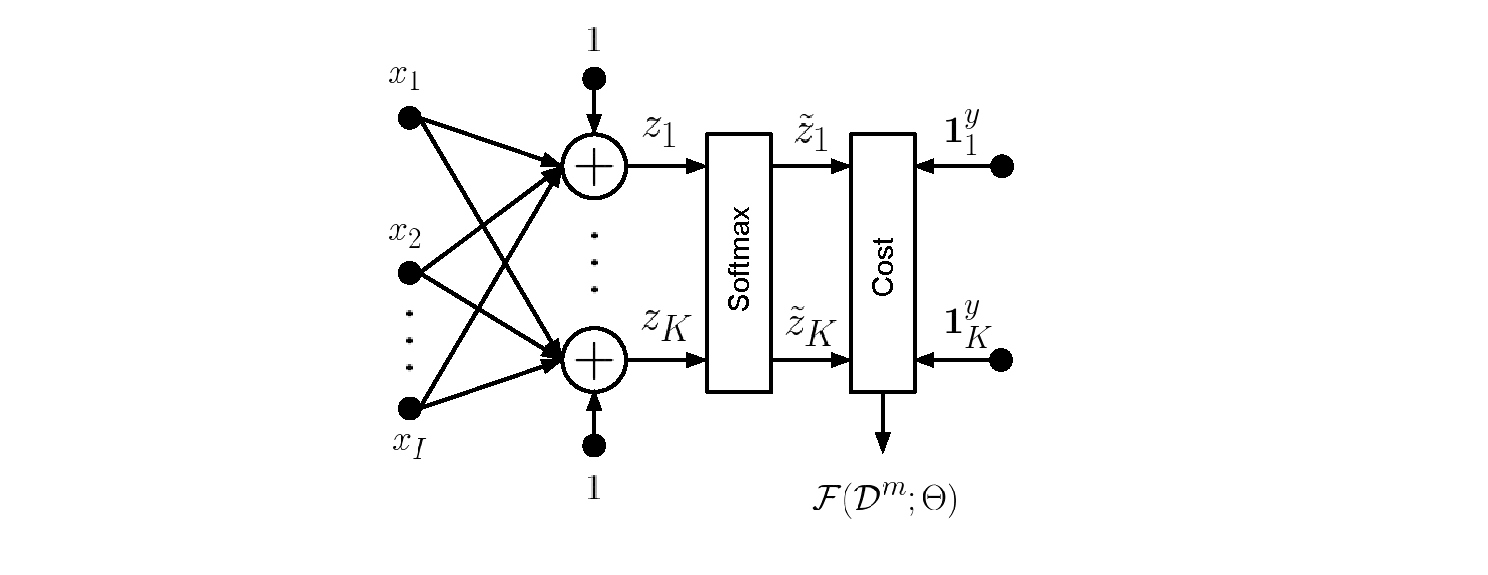
\includegraphics[scale=0.6]{figs/deep_learning/LogLin.pdf}
\caption{Representation of a log-linear model as a computation graph: a
composition of linear and non-linear transformations. The classification cost
for the $m$-th training example $\mathcal{D}^m=\{\mathbf{x}, y\}$ is also
shown. Note $\mathbf{1}^y$ is an indicator vector with a one in position $y$.} 
\label{fig:LogLinear}
\end{figure}

A computation graph is just a way of expressing a multi-input multi-output
function with a directed acyclic graph. Each node in the graph applies a
function over the outputs of its parent nodes and passes the result to its child-nodes,
thus attaining very complex functions by \textit{composing} simpler functions.
To introduce the concept we will work with a very simple example, a categorical
distribution over $K$ classes parametrized as a log-linear model. This is given
by
%
\begin{align}
p(y=k|{x}) & = \frac{1}{Z(\mathbf{W},\mathbf{b},\mathbf{x})}\exp\left(\sum_{i=1}^{I} W_{ik} x_i + b_k\right),
\label{eq:loglineargen}
\end{align}
%
\noindent where 
\begin{align}
Z(\mathbf{W},\mathbf{b},\mathbf{x}) = \sum_{k'=1}^{K} \exp\left(\sum_{i=1}^{I} W_{ik'} x_i + b_{k'}\right)
\label{eq:loglineargenPartition}
\end{align}
%
is the partition function ensuring that all output values sum to one, so that we can interpret
these values as probabilities. The model thus receives a feature vector
$\mathbf{x} \in \mathbb{R}^{I}$ and assigns a probability over $y \in {1 \cdots K}$ possible
class indices. It is parametrized by weights and bias $\Theta=\{\mathbf{W},
\mathbf{b}\}$, with $\mathbf{W} \in \mathbb{R}^{K \times J}$ and $\mathbf{b}
\in \mathbb{R}^{K}$. This is a well known classifier bearing resemblance to the
models seen in the second day of the school, in
particular the maxent model\footnotemark\footnotetext{There are some
differences with respect to Eq.\ref{eq:loglinear}, like the use of a bias
$\mathbf{b}$. Also, if we consider the binary joint feature mapping
$\boldsymbol{f}(x,y) = \boldsymbol{g}(x) \otimes \boldsymbol{e}_y\nonumber$ of
Eq.\ref{eq:jointfeatsimple}, the maximum entropy classifier in
Eq.\ref{eq:loglinear} becomes a special case of Eq.\ref{eq:loglineargen}, in
which the feature vector $\mathbf{x}$ only take binary values and the bias
parameters in $\mathbf{b}$ are all set to zero.}. 

Another way of looking at these models is as the composition of the linear transformation 
%
\begin{equation}
    z_k = \sum_{i=1}^{I} W_{ik} x_i + b_k,
\label{eq:linear}
\end{equation}
%\begin{equation}
%\mathbf{z} = \mathbf{W} \cdot \mathbf{x} + \mathbf{b},
%\label{eq:linear}
%\end{equation}
%
with the \textit{softmax} non-linear transformation

\begin{equation}
p(y=k|{x}) \equiv \tilde{z}_k = \frac{\exp(z_k)}{\sum_{k'=1}^{K} \exp(z_{k'})}.
\label{eq:softmax}
\end{equation}

This is shown as a computation graph in Fig.~\ref{fig:LogLinear}. Note that in
the following sections we will also use $\mathbf{z}$ and $\tilde{\mathbf{z}}$
to denote the output of linear and non-linear functions respectively.

\subsection{Stochastic Gradient Descent: a refresher}

As we saw on day one, the parameters of a log linear model
$\Theta=\{\mathbf{W}, \mathbf{b}\}$ can be learned with Stochastic Gradient Descent (SGD). To apply SGD we first need to define an error function that measures how
good we are doing for any given parameter values. %.
 To remain close to the maximum
entropy example, we will use as cost function the average minus posterior probability of
the correct class, also known as the Cross-Entropy (CE) criterion. Bear in
mind, however, that we could pick other non-linear functions and cost functions
that do not have
a probabilistic interpretation. For example, the same principle could be applied to
a regression problem where the cost is the Mean Square Error (MSE).

For a training data-set $\mathcal{D} = \{(\mathbf{x}^1,y^1), \ldots,
(\mathbf{x}^M,y^M)\}$ of $M$ examples, the CE cost function is given by

\begin{align}
\mathcal{F}(\mathcal{D};\Theta) 
& = -\frac{1}{M}\sum_{m=1}^{M} \log p(y^m=k(m) | \mathbf{x}^m),
\label{eq:CostLogPos}
\end{align}
% \nonumber\\&= -\frac{1}{M}\sum_{m=0}^{M-1} (\log \circ f_{k(m)} \circ \mathbf{g})(\mathbf{x}^m^)
%
where $k(m)$ is the correct class index for the $m$-th example.
To learn the parameters of this model with SGD, all we need to do is compute the gradient
of the cost $\nabla\mathcal{F}$ with respect to the parameters of the model and
iteratively update our  parameter estimates as 

\begin{equation}
\mathbf{W} \leftarrow \mathbf{W} - \eta \nabla_\mathbf{W}\mathcal{F}
\end{equation}
and
\begin{equation}
\mathbf{b} \leftarrow \mathbf{b} - \eta \nabla_\mathbf{b}\mathcal{F},
\end{equation}

\noindent where $\eta$ is the learning rate. Note that in practice we will use
a mini-batch of examples as opposed to the whole train set. Very often, more
elaborated learning rules as e.g. momentum or Adagrad are used. Bear in mind
that, in general, these still require the computation of the gradients as the
main step. The reasoning here outlined will also be applicable to these.  

\subsection{Deriving Gradients in Computation Graphs using the Chain Rule}

\begin{figure}[!h]
\centering
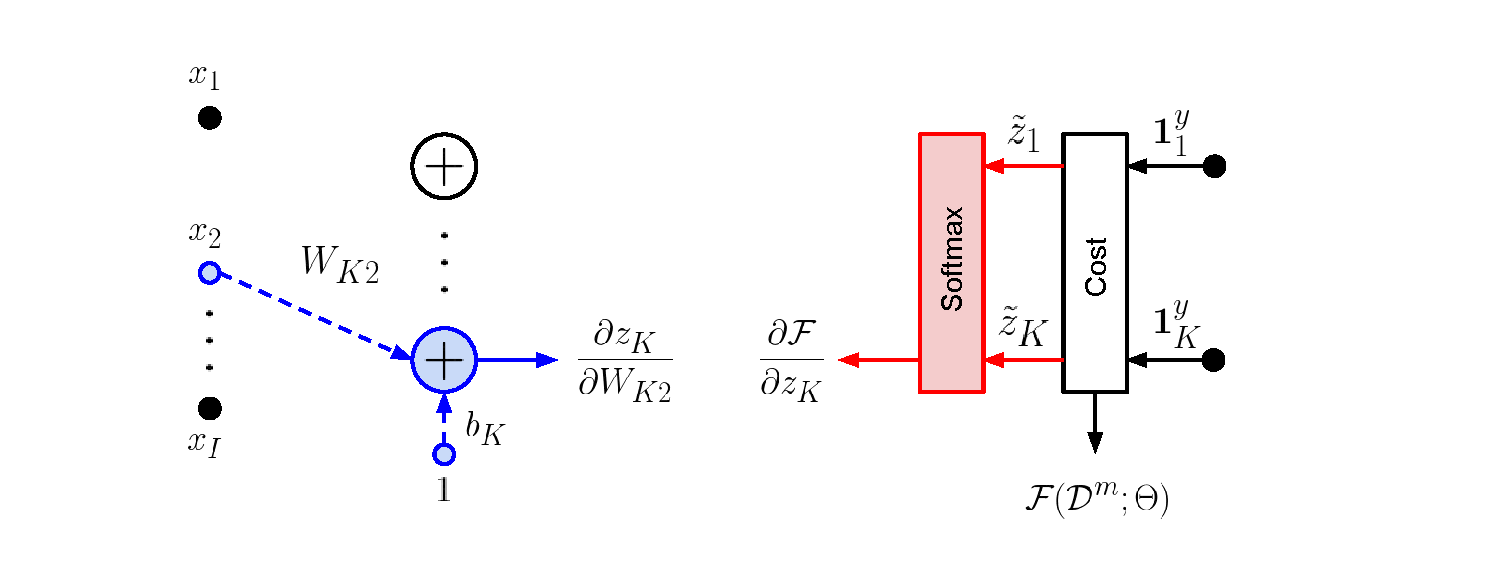
\includegraphics[scale=0.6]{figs/deep_learning/LogLin_color.pdf}
\caption{Forward-pass (blue) and Backpropagation (red) calculations to estimate the gradient of weight $W_{K2}$ and bias $b_K$ of a log-linear model.}
\label{fig:LogLinColor}
\end{figure}

The expressions for $\nabla\mathcal{F}$ are well known in the case of log-linear models. However, for
the sake of the introduction to deep learning, we will show how they can
be derived by exploiting the decomposition of the cost function into the computational
graph seen in the last section (and represented in Fig.~\ref{fig:LogLinear}). To simplify notation, and without loss of generality, we will work with the 
classification cost of an individual example 
%
\begin{align}
\mathcal{F}(\mathcal{D}^m;\Theta) 
= -\log p(y^m=k(m) | \mathbf{x}^m), 
\label{eq:CostLogPosExample}
\end{align}
%
where $\mathcal{D}^m=\{(\mathbf{x}^m, y^m)\}$. Due to linearity, extending the
gradients of \ref{eq:CostLogPosExample} to $M$ examples as in
\ref{eq:CostLogPos} simply implies computing the average of the gradients for
the individual examples. That is

% DAVID: A formula is worth a lot of words

\begin{align}
\nabla_\mathbf{W}\mathcal{F}(\mathcal{Dˆm};\Theta) = - \frac{1}{M} \sum_{m=1}ˆM \nabla_\mathbf{W} \log p(y^m=k(m) | \mathbf{x}^m)
\label{eq:GradientCostDecomposition}
\end{align}

All we need to do to compute $\nabla_\mathbf{W}\mathcal{F}(\mathcal{D};\Theta)$  is to have an expression for $\nabla_\mathbf{W} \log p(y^m=k(m) | \mathbf{x}^m)$.

% RAMON: This might need to be clarified
%Also in a slight abuse of notation we will denote the derivative of the cost
%with respect to an intermediate variable of the graph $z$ as
%\begin{align}
% \frac{\partial \mathcal{F}(\mathcal{D}^m;\Theta)}{\partial z}
%\end{align}

Lets start by computing the element $(k,i)$ of the matrix gradient
$\nabla_\mathbf{W}\mathcal{F}(\mathcal{Dˆm};\Theta)$, which contains the partial
derivative with respect to the weight $W_{ki}$. To do this, we invoke the \textbf{chain rule} to split the derivative calculation into two terms at variable $z_{k'}$ (Eq.\ref{eq:linear}) with $k'=1\cdots K$
%
\begin{align}
\frac{\partial \mathcal{F}(\mathcal{Dˆm};\Theta)}{\partial W_{ki}} & = \sum_{k'=1}^{K} { \color{red} \frac{\partial \mathcal{F}(\mathcal{Dˆm};\Theta)}{\partial z_{k'}} }{ \color{blue} \frac{\partial z_{k'}}{\partial W_{ki}}}.
\label{eq:LogLingCR1}
\end{align}
%
We have thus transformed the problem of computing the derivative into computing two easier derivatives. Since $z_{k'}$ only depends on the weight $W_{ki}$ in a linear way (see the graph in Fig.~\ref{fig:LogLinColor}), the second derivative in Eq.\ref{eq:LogLingCR1} is given by
\begin{align}
\frac{\partial z_{k'}}{\partial W_{ki}} = \frac{\partial }{\partial W_{ki}}\left(\sum_{i'=1}^{I} W_{k'i'} xˆm_{i'} + b_{k'} \right) = 
  &\begin{cases}
      x_i^m  &  \mbox{ if } k = k'\\ 
      0    &  \mbox{ otherwise },
  \end{cases}
  \label{eq:partialLinear}
\end{align}
%
\noindent which implies that 
%
\begin{align}
\frac{\partial \mathcal{F}(\mathcal{D}^m;\Theta)}{\partial W_{ki}} = \frac{\partial \mathcal{F}(\mathcal{D}^m;\Theta) }{\partial z_k} x_i .
\label{eq:gradlogPycx}
\end{align}
%
\noindent The first term derivative is given by
%
\begin{align}
\frac{\partial \mathcal{F}(\mathcal{D}^m;\Theta)}{\partial z_{k}} = \frac{\partial }{\partial z_{k}}\left(z_k - \log\left(\sum_{k'=1}^{K} \exp(z_{k'}) \right) \right) = 
  \begin{cases}
      1 - \tilde{z}_k  &  \mbox{ if } k = k(m)\\ 
      -\tilde{z}_k    &  \mbox{ otherwise }.
  \end{cases}
  \label{eq:patialSoftmax}
\end{align}
%
From the formula for each element and a single example, we can now obtain the gradient matrix for a batch of $M$ examples by simply averaging and expressing the previous equations in vector form as follows
\begin{equation}
\nabla_\mathbf{W}\mathcal{F}(\mathcal{D};\Theta) = -\frac{1}{M}\sum_{m=1}^{M} \Big(\mathrm{\mathbf{1}}^{y^m} - \tilde{\mathbf{z}}^m \Big) \left(\mathbf{x}^m\right)^T.
\label{gradWeigths}
\end{equation}
%
Here $\mathrm{\mathbf{1}}^{y^m} \in \mathbb{R}^{K}$ is a vector of zeros with a one in $y^m=k(m)$, which is 
the index of the correct class for the example $m$. 

In order to compute the derivatives of the cost function with respect to the
bias parameters $b_{k}$, we only need to compute one additional derivative
\begin{align}
\frac{\partial z_{k'}}{\partial b_{k}} = 
  &\begin{cases}
      1  &  \mbox{ if } k = k'\\ 
      0  &  \mbox{ otherwise }.
  \end{cases} 
  \label{eqn:eqsilonq}
\end{align}
%
This leads us to the last gradient expression

\begin{equation}
\nabla_\mathbf{b}\mathcal{F}(\mathcal{D};\Theta) = -\frac{1}{M}\sum_{m=1}^{M} \Big(\mathrm{\mathbf{1}}^{y^m} - \tilde{\mathbf{z}}^m \Big).
\label{eq:gradBias}
\end{equation}

\noindent An important consequence of the previous derivation is the fact that each 
gradient of the parameters $\nabla_\mathbf{W}\mathcal{F}(\mathcal{D};\Theta)$ and $\nabla_\mathbf{b}\mathcal{F}(\mathcal{D};\Theta)$ can be computed from two terms: 
%
\begin{enumerate}
\item The derivative of the cost with respect to the linear transformation applying the weight $\partial \mathcal{F}(\mathcal{D}^m;\Theta)/\partial z_k$, denoted in \textcolor{red}{red}.
\item The derivative of the forward-pass up to the linear transformation applying the weight $\partial z_k/\partial W_{ik}$, denoted in \textcolor{blue}{blue}. This is always equal to the variable multiplying that weight and one in the case of the bias.
\end{enumerate}
%
\noindent This is the key to the Backpropagation algorithm as we will see in the next Section \ref{sec:deep_forward}.

\section{Going Deeper than Log-linear by using Composition}
\label{sec:deep_forward}

\subsection{The Multilayer Perceptron or Feed-Forward Network}

We have seen that just by using the chain rule we can easily compute gradients for
compositions of two functions (one non-linear and one linear). However, there
was nothing in the derivation that would stop us from composing more than two
functions. Let us think, for example of the following model

\begin{algorithm}[th!]
\label{algo:mlpforward}
   \caption{Forward pass of a Multi-Layer Perceptron (MLP) or Feed-Forward (FF) network\label{alg:mlpforward}}
\begin{algorithmic}[1]

   \STATE {\bfseries input:} Initial parameters for an MLP of $N$ layers $\Theta=\{\mathbf{W}^1, \mathbf{b}^1, \cdots \mathbf{W}^N, \mathbf{b}^N\}$
   \STATE {\bfseries input:} Input data vector $\mathbf{\tilde{z}}^{0}  \equiv \mathbf{x}$. 

	\FOR{$n=1$ {\bfseries to} $N-1$}
     \STATE Apply  linear transformation 
        $$z_j^n = \sum_{i=1}^{I} W_{ji}^n \tilde{z}_i^{n-1} + b_j^n$$
     \STATE Apply non-linear transformation e.g. sigmoid (hereby denoted $\sigma()$)
     $$\tilde{z}_j^n = \sigma(z_j^n)  = \frac{1}{1+\exp(-z_j^n)}$$

	\ENDFOR

\STATE Apply final linear transformation 
   $$z_k^N = \sum_{j=1}^{J} W_{kj}^N \tilde{z}_j^{N-1} + b_k^N$$
\STATE Apply final non-linear transformation e.g. softmax 
$$p(y=k|{x}) \equiv \tilde{z}_k^N = \frac{\exp(z_k^N)}{\sum_{k'=1}^{K} \exp(z_{k'}^N)}$$

\end{algorithmic}
\end{algorithm}

\noindent In a similar fashion to the log-linear model, the MLP/FF can be expressed as a computation graph. This is displayed in Fig.~\ref{fig:FF}

\begin{figure}[!hb]
\centering
%\includegraphics[scale=0.2]{figs/deep_learning/mlp.png}
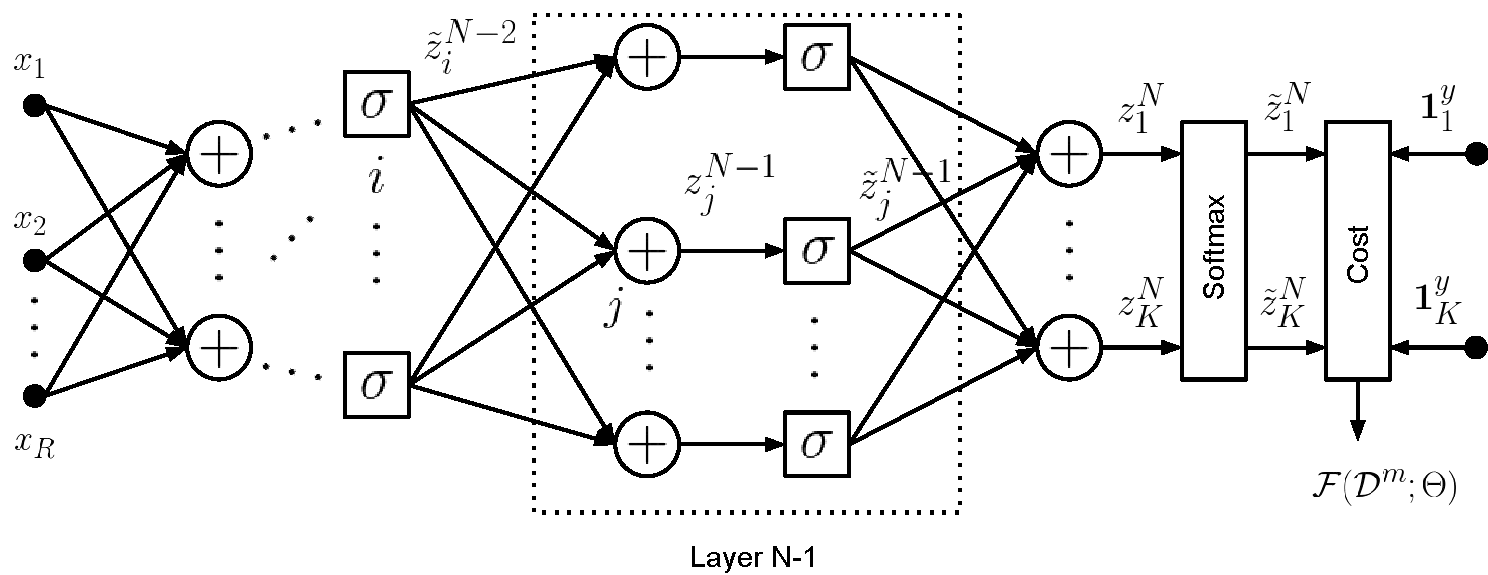
\includegraphics[scale=0.6]{figs/deep_learning/NN.pdf}
\caption{Representation of a Multi-Layer Perceptron (MLP) or Feed-Forward (FF) network as a computation graph. The classification cost
for the $m$-th training example $\mathcal{D}^m=\{\mathbf{x}, y\}$ is also
shown.}
\label{fig:FF}
\end{figure}

\noindent Some considerations:
%
\begin{itemize}
\item MLPs/FFs are characterized by applying functions in a set of layers subsequently to a single input. This characteristic is also shared by convolutional networks, although the latter also have parameter tying constraints.
\item The non-linearities in the intermediate layers are usually one-to-one transformations. The most typical are the sigmoid, hyperbolic tangent and the rectified linear unit (ReLU). 
\item The output non-linearity is determined by the output to be estimated. In order to estimate probability distributions the softmax is typically used. For regression problems a last linear layer is used instead.
\end{itemize}

\subsection{Backpropagation: an overview}

For the examples in this chapter we will consider the case in which we are estimating a distribution over classes. The cost function is thus the same

\begin{align}
\mathcal{F}(\mathcal{D};\Theta) & = -\frac{1}{M}\sum_{m=1}^{M} \log p(y^m=k(m) | \mathbf{x}^m).
\end{align}

To compute the gradient with respect the parameters of the $n$-th layer, we
just need to apply the chain rule as in the previous section, consecutively.
Fortunately, we do not need to repeat this procedure for each layer as it is
easy to spot a recursive rule (the Backpropagation recursion) that is valid
for many neural models, including feed-forward networks (such as MLPs) as well
as recurrent neural networks (RNNs) with minor modifications. The
Backpropagation method, which is given in Algorithm \ref{algo:backprop} for
the case of an MLP, consists of the following steps:

\begin{itemize}
\item The \textcolor{blue}{forward pass} step, where the input signal is injected though the network  in a forward fashion (see Alg.~\ref{algo:mlpforward})
\item The \textcolor{red}{backpropagation} step, where the derivative of the cost function (also called error) is injected back through the network and backpropagated according to the derivative rules (see steps 8-17 in Alg.~\ref{algo:backprop})
\item Finally, the gradients with respect to the parameters are computed by multiplying the input signal from the forward pass and the backpropagated error signal, at the corresponding places in the network (step 18 in Alg.~\ref{algo:backprop})
\item Given the gradients computed in the previous step, the model weights can then be easily update according to a specified learning rule (step 19 in Alg.~\ref{algo:backprop} uses a mini-batch SGD adaptation rule).
\end{itemize}
%Alg.~\ref{algo:backprop} uses a mini-batch SGD updation rule. 

The main step of the method is the backpropagation step, where one has to compute the backpropagation recursion rules for a specific network.
The next section presents a careful deduction of these recursion rules, for the present MLP model. 


\subsection{Backpropagation: deriving the rule}

\begin{figure}[!h]
\centering
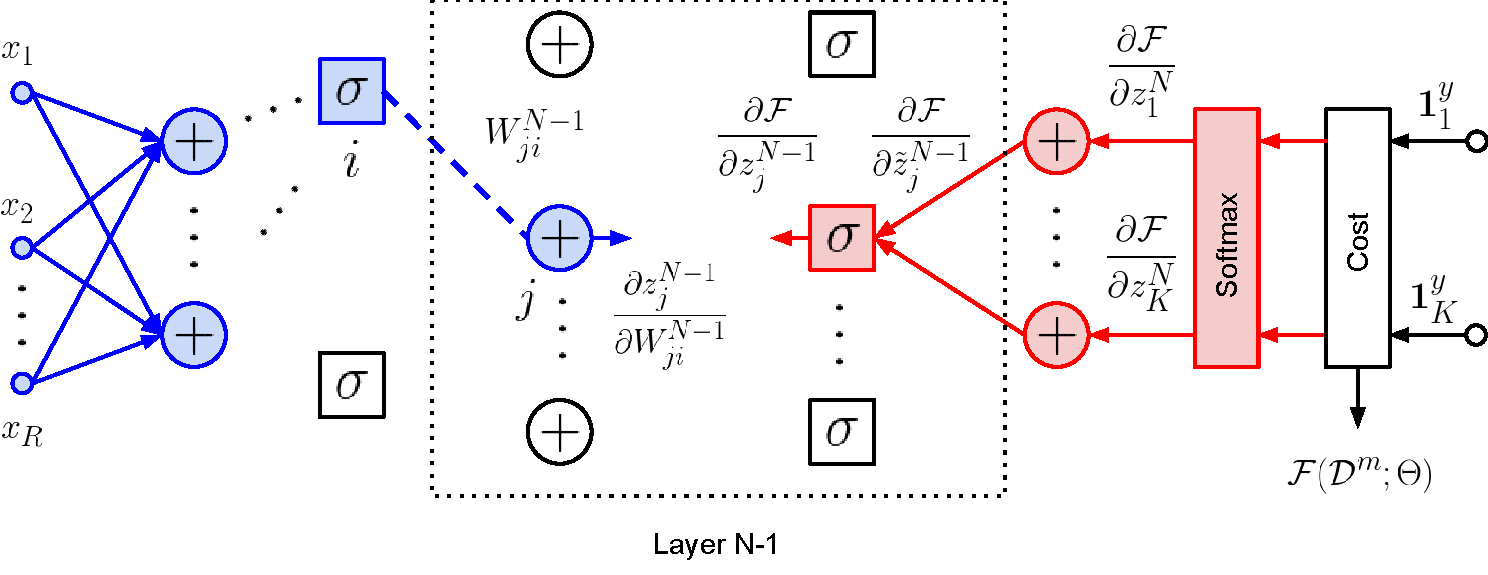
\includegraphics[scale=0.6]{figs/deep_learning/NN_backprop_colored.pdf}
\caption{Forward-pass (blue) and Backpropagation (red) calculations to estimate the gradient of weight $W_{ji}$ at layer $N-1$ of a MLP.}
\label{fig:NN_color}
\end{figure}

In a generic MLP we would like to compute the values of all parameters $\Theta=\{\mathbf{W}^1, \mathbf{b}^1, \cdots \mathbf{W}^N, \mathbf{b}^N\}$. As explained previously, we will thus need to compute the backpropagated error at each node $\partial \mathcal{F}(\mathcal{D}^m;\Theta)/\partial z_k^n$, and the corresponding derivative for the forward-pass $\partial z_k^n/\partial W_{ik}$, for $n = 1 \cdots N$. Fortunately, it is easy to spot a recursion that will allow us to compute these values for each node, given all its child nodes. To spot it, we can start trying to compute the gradients one layer before the output layer (see Fig.~\ref{fig:NN_color}), i.e. layer $N-1$. We start by splitting at $N-1$
%
\begin{align}
\frac{\partial \mathcal{F}(\mathcal{D}^m;\Theta)}{\partial W_{ji}} = \sum_{j'=1}^{J} {\color{red} \frac{\partial \mathcal{F}(\mathcal{D}^m;\Theta)}{\partial z_{j'}^{N-1}}} {\color{blue} \frac{\partial z_{j'}^{N-1}}{\partial W_{ji}}} = {\color{red} \frac{\partial \mathcal{F}(\mathcal{D}^m;\Theta)}{\partial z_{j}^{N-1}}} {\color{blue} \frac{\partial z_{j}^{N-1}}{\partial W_{ji}}}
\label{eq:BPderivation1}
\end{align}
%
where, as in the case of the log-linear model, we have used the fact that only $z_j$ depends on $W_{ji}$. We now advance forward from $z^N_j$ and apply the non-linearity to obtain $\tilde{z}^N_j$. As long as the non-linearity is a one-to-one operation (and this is often the case in neural-networks), we will also get rid of the summation leading to
%
\begin{align}
\frac{\partial \mathcal{F}(\mathcal{D}^m;\Theta)}{\partial W_{ji}} = \bigg(\sum_{j'=1}^{J} \frac{\partial \mathcal{F}(\mathcal{D}^m;\Theta)}{\partial \tilde{z}_{j'}^{N-1}} \frac{\partial \tilde{z}_{j'}^{N-1}}{\partial z_{j}^{N-1}}\bigg) \frac{\partial z_{j}^{N-1}}{\partial W_{ji}}= \frac{\partial \mathcal{F}(\mathcal{D}^m;\Theta)}{\partial \tilde{z}_{j}^{N-1}}\frac{\partial \tilde{z}_{j}^{N-1}}{\partial z_{j}^{N-1}}\frac{\partial z_{j}^{N-1}}{\partial W_{ji}}.
\label{eq:BPderivation2}
\end{align}
%
We will not be so lucky in the next application of the chain rule. Looking at Fig.~\ref{fig:NN_color}, it is clear that the derivatives at each node in layer $N-1$ will depend on all values of layer $N$. We thus have
%
\begin{align}
\frac{\partial \mathcal{F}(\mathcal{D}^m;\Theta)}{\partial W_{ji}} = \bigg(\sum_{k'=1}^{K} \frac{\partial \mathcal{F}(\mathcal{D}^m;\Theta)}{\partial z_{k'}^{N}} \frac{\partial z_{k'}^{N}}{\partial \tilde{z}_{j}^{N-1}}\bigg)\frac{\partial \tilde{z}_{j}^{N-1}}{\partial z_{j}^{N-1}}\frac{\partial z_{j}^{N-1}}{\partial W_{ji}}.
\label{eq:BPderivation3}
\end{align}
%
Now, comparing Eq.~\ref{eq:BPderivation1} with Eq.~\ref{eq:BPderivation3} it is easy to see that, if we denote the derivative of the cost (or error) with respect to the $N$ linear layer of the graph as
%
\begin{align}
e^{N-1} = \frac{\partial \mathcal{F}(\mathcal{D}^m;\Theta)}{\partial z_{k}^{N-1}} ,
\label{eq:BPderivation4}
\end{align}
%
\noindent then we can relate this to the cost derivative with respect to the preceding layer with
%
\begin{align}
e^{N-1} = \bigg(\sum_{k'=1}^{K} e^N \frac{\partial z_{k'}^{N}}{\partial \tilde{z}_{k'}^{N-1}}\bigg)\frac{\partial \tilde{z}_{k'}^{N-1}}{\partial z_{k'}^{N-1}} = \bigg(\sum_{k'=1}^{K} e^N_k W^N_{kj}\bigg)\cdot\tilde{z}_{k'}^{N-1}\cdot(1-\tilde{z}_{k'}^{N-1}),
\end{align}
%
where we have used the fact that for sigmoid non-linearities 
%
\begin{equation}
\frac{\partial \tilde{z}_{k}}{\partial z_{k}} = \tilde{z}_{k}\cdot (1-\tilde{z}_{k}).
\end{equation}

This formula can also be interpreted as traversing the graph in Fig.~\ref{fig:FF} backwards, multiplying at each node the backpropagated error by the derivative of its inputs and summing the errors propagated from different nodes. A more formal expression of the algorithm can be found in Algorithm~\ref{algo:backprop}.

\begin{algorithm}[th!]

   \caption{Mini-batch SGD with Back-Propagation}

\begin{algorithmic}[1]
\label{algo:backprop}

   \STATE {\bfseries input:} 
   %Data $\mathcal{D}$, Feed-forward of $N$ layers, with parameters $\Theta=\{\mathbf{W}^1, \mathbf{b}^1, \cdots \mathbf{W}^N, \mathbf{b}^N\}$, number of rounds $T$, $B$ mini-batches of size $M$, learning rate $\eta$
Data $\mathcal{D}=\{\mathcal{D}_1,\mathcal{D}_2,...,\mathcal{D}_B\}$ split into $B$ mini-batches of size $M'$%(in each data mini-batch $\mathcal{D}_b$ the example indicies $m$ range from 1 to $M'$)
, MLP of $N$ layers, with parameters $\Theta=\{\mathbf{W}^1, \mathbf{b}^1, \cdots \mathbf{W}^N, \mathbf{b}^N\}$, number of rounds $T$, learning rate $\eta$

   \STATE initialize parameters $\Theta$ randomly 

	\FOR{$t=1$ {\bfseries to} $T$}
	\FOR{$b=1$ {\bfseries to} $B$}

	\vspace{0.3cm}
	\FOR{$m=1$ {\bfseries to} $M'$}
	\STATE Compute the {forward pass} for each of the $M'$ examples in batch $b$:
	 and keep not only $p(y^m|\mathbf{x}^m) \equiv \tilde{\mathbf{z}}^{m,N}$ and all intermediate non-linear outputs $\tilde{\mathbf{z}}^{m,1} \cdots \tilde{\mathbf{z}}^{m,N}$.
	\ENDFOR	
	\vspace{0.3cm}
    %\STATE \textbf{Backpropagate} $\nabla_{\mathbf{z}^{m,n}}\mathcal{F}(\mathcal{D}_b;\Theta)$ 
	\FOR{$n=N$ {\bfseries to} $1$}
        \IF{n==N} 
		\FOR{$m=1$ {\bfseries to} $M'$}
        \STATE {Initialize the error at last layer, for each example $m$. For the softmax with CE cost this is given by:
        $$\mathbf{e}^{m,N} = \Big(\mathrm{\mathbf{1}}_{k(m)} - \tilde{\mathbf{z}}^{m,N} \Big).$$}
		\ENDFOR	
        \ELSE
   		\FOR{$m=1$ {\bfseries to} $M'$}
		\STATE {Backpropagate} the error through the linear layer, for each example $m$:  
        $$\mathbf{e}^{m,n} = \Big((\mathbf{W}^{n+1})^T \mathbf{e}^{m,n+1}\Big)$$ 
        
		\STATE {Backpropagate} the error through the non-linearity, for the sigmoid this is:  
        $$\mathbf{e}^{m,n} = \mathbf{e}^{m,n+1} \odot \tilde{\mathbf{z}}^{m,n} \odot (\mathbf{\mathrm{1}}-\tilde{\mathbf{z}}^{m,n}),$$
        where $\odot$ is the element-wise product and the $\mathbf{\mathrm{1}}$ is replicated to match the size of $\tilde{\mathbf{z}}^n$.


		\ENDFOR	
        \ENDIF 

		\vspace{0.3cm}
        \STATE {Compute the gradients} using the backpropagated errors and the inputs from the forward pass

        $$\nabla_{\mathbf{W}^n}\mathcal{F}(\mathcal{D_b};\Theta)  = -\frac{1}{M'} \sum_{m=1}^{M'} \mathbf{e}^{m,n} \cdot \left(\tilde{\mathbf{z}}^{m,n-1}\right)^T,$$ 
        $$\nabla_{\mathbf{b}^n}\mathcal{F}(\mathcal{D_b};\Theta)  = - \frac{1}{M'} \sum_{m=1}^{M'} \mathbf{e}^{m,n}.$$  

		\vspace{0.3cm}
        \STATE Update the parameters 
            $$\mathbf{W}^n \leftarrow \mathbf{W}^n - \eta \nabla_\mathbf{W^n}\mathcal{F},$$ 
            $$\mathbf{b}^n \leftarrow \mathbf{b}^n - \eta \nabla_\mathbf{b^n}\mathcal{F}.$$ 

	\ENDFOR

	\ENDFOR
	\ENDFOR
\end{algorithmic}
\end{algorithm}

\clearpage

\begin{exercise}
Go to lxmls/deep\_learning/mlp.py:class NumpyMLP:def grads() and complete the
code of the NumpyMLP class with the Backpropagation recursion that we just saw.
Once you are done. Try different network geometries by increasing the number of
layers and layer sizes e.g.
\begin{python}
# Model parameters
geometry = [train_x.shape[0], 20, 2]
actvfunc = ['sigmoid', 'softmax'] 
# Instantiate model
mlp      = dl.NumpyMLP(geometry, actvfunc) 
\end{python}
You can test the different models with the same sentiment analysis problem as
in Exercise 6.1. 
\begin{python}
# Model parameters
n_iter = 5
bsize  = 5
lrate  = 0.01
# Train
sgd.SGD_train(mlp, n_iter, bsize=bsize, lrate=lrate, train_set=(train_x, train_y))
acc_train = sgd.class_acc(mlp.forward(train_x), train_y)[0]
acc_test  = sgd.class_acc(mlp.forward(test_x), test_y)[0]
print "MLP (%s) Amazon Sentiment Accuracy train: %f test: %f" % (geometry, acc_train,acc_test)
\end{python}
\end{exercise}

\subsection{Some final reflections on Backpropagation}

If you are new to the neural network topic, this is about the most important
piece of theory you should learn about deep learning. Here are some reflections
that you should keep in mind.

\begin{itemize}
\item Thanks to the multi-layer structure and the chain rule, Backpropagation allows models that compose linear and non-linear functions with any depth (in principle\footnotemark). 

\item The formulas are also valid for other cost functions and output layer non-linearities with minor modifications. It is only necessary to compute the equivalente of Eq.~\ref{eq:patialSoftmax}. 

\item The formulas are also valid for hidden non-linearities other than the sigmoid. Element-wise non-linear transformations still allow the simplification in Eq.~\ref{eq:chainRulRecursion}. With little effort it is also possible to deal with other cases.

\item However, there is an important limitation: unlike the log-linear models, the optimization problem is \textit{non convex}. This removes some formal guarantees, most importantly we can get trapped in local minima during training.
\end{itemize}

\footnotetext{Not exactly, since it is possible to run into numerical problems.}

% THIS WILL BE COMMENTED UNTIL THE FINAL UPDATE
%
%\subsection{A Note on Pre-Trainining}
%
%If you already have some experience with neural networks you might have
%realised that all what we show here is classic MLP theory, which is 30-40 years
%old. Indeed, it could be argued that, at the core, many modern deep learning
%applications are just classical neural networks theory with more data and more
%computing power. One of the novelties that came along the deep learning wave of
%research is pre-training with the Restricted Boltzmann Machine (RBM) paradigm.
%The cost function for a MLP of many layers becomes too complex and, as
%mentioned before, local minima and non-convexity make training of deep MLPs
%problematic. 
%
%The RBM paradigm allows to pre-train a MLP in \textit{unsupervised} fashion
%i.e. with out reference labels $\mathbf{y}^m$, which has been shown to improve
%posterior training. However, current state of the art systems do not always use
%RBM pre-training, resort to simpler types of smart-initializations or use none.
%Fort his reason, we will only see pre-training as an advance topic.  

%%%%%%%%%%%%%%%%%%%%%%%%%%%%%%%%%%%%%%%%%%%%%%%%%%%%%
\section{Deriving gradients and GPU code with Theano}
%%%%%%%%%%%%%%%%%%%%%%%%%%%%%%%%%%%%%%%%%%%%%%%%%%%%%

\subsection{An Introduction to Theano}

As you may have observed, the speed of SGD training for MLPs slows down
considerably when we increase the number of layers. One reason for this is that
the code that we use here is not very optimized. It is thought for you to
learn the basic principles. Even if the code was more optimized, it would still be
very slow for reasonable network sizes. The cost of computing each
linear layer is proportional to the dimensionality of the previous and current
layers, which in most cases will be rather large. 

For this reason most deep learning applications use Graphics Processing Units
(GPU) in their computations. This specialized hardware is normally used to
accelerate computer graphics, but can also be used for general computation
intensive tasks. However, we need to deal with specific interfaces and
operations in order to use a GPU. This is where Theano comes in. Theano is a
multidimensional symbolic expression python module with focus on neural
networks. It will provide us with the following nice features:

\begin{itemize}
\item Symbolic expressions: Express the operations of the MLP (forward pass, cost) symbolically, as mathematical operations rather than explicit code 
\item Symbolic Differentiation: As a consequence of the previous feature, we can compute gradients of arbitrary mathematical functions automatically.   
\item GPU integration: The code will be ready to work on a GPU, provided that you have one and it is active within Theano. It will also be faster on normal CPUs since the symbolic operations are compiled to C code. 
\item Theano is focused on Deep Learning, with an active community and several tutorials easily available.  
\end{itemize}

The only negative aspect is that we will have to learn to deal with Theano and
in particular working with symbolic representations. We will start right away
with some exercises.

\begin{exercise}
Get in contact with Theano. Learn the difference between a symbolic
representation and a function. Start by implementing the first layer of our
previous MLP in Numpy 
\begin{python}
# Numpy code
x        = test_x             # Test set 
W1, b1   = mlp.params[:2]     # Weights and bias of fist layer 
z1       = np.dot(W1, x) + b1 # Linear transformation
tilde_z1 = 1/(1+np.exp(-z1))  # Non-linear transformation  
\end{python}
Now we will implement this in Theano.  We start by creating the variables over
which we will produce the operations. For example the symbolic input is defined
as
\begin{python}
# Theano code. 
# NOTE: We use undescore to denote symbolic equivalents to Numpy variables. 
# This is no Python convention!.
import theano
import theano.tensor as T
_x = T.matrix('x')
\end{python}
Note that this variable does not have any particular value, nor a space
reserved in memory for it. It contains just a symbolic definition of what the
variable can contain. The particular values will be given when we use it to
compile a function. 

We could actually use the same definition format to define the weights and give
their particular values as inputs to the compiled function. However, since we
will be using a more complicated format in later exercises, we will use it here
as well. The \textit{shared} class allows to define variables that are shared
across functions. They are also given a concrete value so that we do not need
to give it for each function call. This format is therefore ideal for the
weights of our network.
\begin{python}
_W1 = theano.shared(value=W1, name='W1', borrow=True) 
_b1 = theano.shared(value=b1, name='b1', borrow=True, broadcastable=(False, True)) 
\end{python}
Now lets describe the operations we want to do with the variables. Again only
symbolically. This is done by replacing our usual operations by Theano symbolic
ones when necessary e. g. the internal product dot() or the sigmoid. Some
operations like e.g. $+$ are automatically recognized by Theano (operator
overloading). 
\begin{python}
_z1            = T.dot(_W1, _x) + _b1
_tilde_z1      = T.nnet.sigmoid(_z1)
# Keep in mind that naming variables is useful when debugging
_z1.name       = 'z1'
_tilde_z1.name = 'tilde_z1'
\end{python}
When debugging the code it is often useful to print the graph of computations.
\begin{python}
# Perceptron computation graph
theano.printing.debugprint(_tilde_z1)

sigmoid [@A] 'tilde_z1'
 |Elemwise{add,no_inplace} [@B] 'z1'
   |dot [@C] ''
   | |W1 [@D]
   | |x [@E]
   |b1 [@F]

\end{python}
It is important to keep in mind that, until this point, we do not have a
function we can use to produce any practical input. In order to obtain this we
have to compile this function by calling    
\begin{python}
layer1 = theano.function([_x], _tilde_z1)
\end{python}
Note the use of $[$ $]$ for the input variables, even if we just specify one
variable. We can now do a test to compare the Numpy and Theano implementations
and see that they give the same outputs.
\begin{python}
# Check Numpy and Theano match
if np.allclose(tilde_z1, layer1(x.astype(theano.config.floatX))):
    print "\nNumpy and Theano Perceptrons are equivalent"
else:
    raise ValueError, "Numpy and Theano Perceptrons are different"
\end{python}
\end{exercise}

\subsection{Symbolic Forward Pass}
In the previous section you have seen how to create symbolic Theano functions
with shared parameters. You have thus all you need to implement the whole
forward pass of a generic MLP in Theano.
\begin{exercise}
Complete the method \_forward() inside of the lxmls/deep\_learning/mlp.py:class
TheanoMLP. Note that this is called only once at the initialization of the
class. To debug your implementation put a breakpoint at the \_\_init\_\_
function call. Hint: Note that this is very similar to NumpyMLP.forward().
You just need to keep track of the symbolic variable representing the output of
the network after each layer is applied and compile the function at the end.
After you are finished instantiate a Theano class and check that Numpy and
Theano forward pass are the same. 

\begin{python}
mlp_a = dl.NumpyMLP(geometry, actvfunc)
mlp_b = dl.TheanoMLP(geometry, actvfunc)
\end{python}

Bear in mind that you can use previous experience to debug this.

\end{exercise}

\subsection{Symbolic Differentiation}
In the previous section we compiled the forward pass of a MLP. In this section
we will do the same with the cost used for training. We will also derive the
gradients although this will be trivial once we have the cost function compiled.     
\begin{exercise}
We first see an example that does not use any of the code in TheanoMLP but
rather continues from what you wrote in exercise 6.3. In this exercise you
completed a sigmoid layer with Theano. To get some values for the weights we
used the first layer of the network you trained in 6.2. now we are going to use
the second layer as well. This is thus assuming that your network in 6.2 has
only two layers e.g. the recommended geometry (I, 20, 2). Make sure this is the
case before starting this exercise.  

For the sake of clarity, lets write here the part of Ex. 6.2 that we had completed
\begin{python}
# Get the values from our MLP from Ex 6.2
W1, b1   = mlp.params[:2]     # Weights and bias of fist layer 
# First layer symbolic variables
_x  = T.matrix('x')
_W1 = theano.shared(value=W1, name='W1', borrow=True) 
_b1 = theano.shared(value=b1, name='b1', borrow=True, broadcastable=(False, True)) 
# First layer symbolic expressions
_z1       = T.dot(_W1, _x) + _b1
_tilde_z1 = T.nnet.sigmoid(_z1)
\end{python}
Now we just need to complete this with the second layer, using a softmax non-linearity
\begin{python}
W2, b2  = mlp.params[2:]     # Weights and bias of second (and last!) layer 
# Second layer symbolic variables
_W2 = theano.shared(value=W2, name='W2', borrow=True) 
_b2 = theano.shared(value=b2, name='b2', borrow=True, broadcastable=(False, True)) 
# Second layer symbolic expressions
_z2       = T.dot(_W2, _tilde_z1) + _b2
_tilde_z2 = T.nnet.softmax(_z2.T).T
\end{python}
With this, we could compile a function to obtain the output of the network
symb\_tilde\_z2 for a given input symb\_x. In this exercise we are however
interested in obtaining the misclassification cost. This is given in Eq:
\ref{eq:CostLogPos}. First we are going to need the symbolic variable for the
correct output
\begin{python}
_y = T.ivector('y')
\end{python}
The minus posterior probability of the class given the input is the same as
selecting the $k(m)$-th softmax output, were $k(m)$ is the index of the correct
class for $x^m$. If we want to do this for a vector $\mathbf{y}$ containing $M$
different examples, we can write this as
\begin{python}
_F = -T.mean(T.log(_tilde_z2[_y, T.arange(_y.shape[0])]))
\end{python}
Now obtaining a function that computes the gradient could not be easier.
\begin{python}
_nabla_F = T.grad(_F, _W1) 
nabla_F  = theano.function([_x, _y], _nabla_F) 
\end{python}
To finish this exercise have a look at the TheanoMLP class. As you may realise it just implements what is shown above for the generic case of $N$ layers
\end{exercise}

\subsection{Symbolic mini-batch update}

The code above is used in the normal SGD\_train when utilizing Theano. Even if
you do not have a GPU configured, it should be run faster than our Numpy
version, particularly for large batch sizes. There is however a
way to make it run even faster by implementing not only gradient computation
but the whole batch update of SGD inside Theano. For this we need also to share
the whole training set, or a very large mega-batch of it. 

\begin{exercise}
Let us first have an understanding of handling train/test data inside the Theano
computation graph. One important aspect to take into account is that both type
and shape of the data have to match their corresponding graph variables. This is
the main source of errors when you are starting with Theano. 
\begin{python}
# Cast data into the types and shapes used in the Theano graph
train_x = train_x.astype(theano.config.floatX)
train_y = train_y.astype('int32')
\end{python}
Note the Theano type theano.config.floatX. This will automatically switch
between float32 (GPU) and float64 (CPU).

To use data in a Theano computation graph, we use the theano.shared variable.
This will also push data into the GPU, if used.
\begin{python}
_train_x = theano.shared(train_x, 'train_x', borrow=True)
_train_y = theano.shared(train_y, 'train_y', borrow=True)
\end{python}
Once this is done, we can create and compile functions using these variables.
One simple but useful function is a function returning a mini-batch of data 
of size bsize given the mini-batch index.  
\begin{python}
_i             = T.lscalar()
get_tr_batch_y = theano.function([_i], _train_y[_i*bsize:(_i+1)*bsize]) 
\end{python}
Compile this function and observe its behaviour. It will be necessary for the next exercise.
\end{exercise}

\begin{exercise}
The mini-batch function in the previous exercise is the key to fast batch
update. This is combined with the \emph{updates} argument of theano.function. The input to this argument,
is a list of tuples with each parameter and update rule. This can be compactly
defined using list comprehensions.
\begin{python}
mlp_c   = dl.TheanoMLP(geometry, actvfunc)
_x      = T.matrix('x')
_y      = T.ivector('y')
_F      = mlp_c._cost(_x, _y)
updates = [(par, par - lrate*T.grad(_F, par)) for par in mlp_c.params]
\end{python}

This can be now combined with the givens argument of theano.function. This maps
input and target to other variables. In this case a mini-batch of inputs and
targets given an index. 
\begin{python}
_j      = T.lscalar()
givens  = { _x : _train_x[:, _j*bsize:(_j+1)*bsize], 
            _y : _train_y[_j*bsize:(_j+1)*bsize] }
\end{python}

With updates and givens, we can now define the batch update function. This will
return the cost of each batch and update the MLP parameters at the same time
using updates
\begin{python}
batch_up = theano.function([_j], _F, updates=updates, givens=givens)
n_batch  = train_x.shape[1]/bsize  + 1
\end{python}
Once we have defined this, we can compare speed and accuracy of the Numpy
and simple gradient versions using

\begin{python}
import time
# Model
geometry = [train_x.shape[0], 20, 2]
actvfunc = ['sigmoid', 'softmax'] 

# Numpy MLP
mlp_a     = dl.NumpyMLP(geometry, actvfunc)
init_t    = time.clock()
sgd.SGD_train(mlp_a, n_iter, bsize=bsize, lrate=lrate, train_set=(train_x, train_y))
print "\nNumpy version took %2.2f sec" % (time.clock() - init_t)
acc_train = sgd.class_acc(mlp_a.forward(train_x), train_y)[0]
acc_test  = sgd.class_acc(mlp_a.forward(test_x), test_y)[0]
print "Amazon Sentiment Accuracy train: %f test: %f\n" % (acc_train, acc_test)

# Theano grads 
mlp_b  = dl.TheanoMLP(geometry, actvfunc)
init_t = time.clock()
sgd.SGD_train(mlp_b, n_iter, bsize=bsize, lrate=lrate, train_set=(train_x, train_y))
print "\nCompiled gradient version took %2.2f sec" % (time.clock() - init_t)
acc_train = sgd.class_acc(mlp_b.forward(train_x), train_y)[0]
acc_test  = sgd.class_acc(mlp_b.forward(test_x), test_y)[0]
print "Amazon Sentiment Accuracy train: %f test: %f\n" % (acc_train, acc_test)

# Theano batch update
init_t = time.clock()
sgd.SGD_train(mlp_c, n_iter, batch_up=batch_up, n_batch=n_batch)
print "\nTheano compiled batch update version took %2.2f" % (time.clock() - init_t)
acc_train = sgd.class_acc(mlp_c.forward(train_x), train_y)[0]
acc_test  = sgd.class_acc(mlp_c.forward(test_x), test_y)[0]
print "Amazon Sentiment Accuracy train: %f test: %f\n"%(acc_train,acc_test)
\end{python}
As you may observe, just computing the gradients with Theano may not lead to
a decrease, but rather an increase in computing time. To maximally exploit
the power of Theano, it is necessary to bundle both computations and data 
together using approaches like the compiled batch update.
\end{exercise}
